\section{汇编语言简介}

\begin{frame}\ft{机器语言}
  \begin{defn}{}
    机器语言是机器指令的集合。机器指令是计算机可以正确执行的命令,它是一组二进制数字。计算机将其转变为一组高低电平,以使电子器件收到驱动,进行运算。
  \end{defn}
  \pause
  
  \begin{exam}{}
    8086CPU完成运算$s=768+12288-1280$的机器码如下:
    $$
    \begin{array}{c}
      1011~0000~0000~0000~0000~0011\\
      0000~0101~0000~0000~0011~0000\\
      0010~1101~0000~0000~0000~0101
    \end{array}
    $$
    \pause
    若将程序错写成以下形式,请指出错误:
    $$
    \begin{array}{c}
      1011~0000~0000~0000~0000~0011\\
      0000~0101~0000~0000~0011~0000\\
      0001~0110~1000~0000~0000~0101
    \end{array}
    $$
  \end{exam}
\end{frame}

% \begin{frame}\ft{机器语言}
%   由此可见,编写和阅读机器码程序不是一件简单的工作,需要记住抽象的二进制码。上面只是一个非常简单的小程序,就暴露了机器码的晦涩难懂和不易查找。\vspace{0.1in}

%   早期程序员很快发现了使用机器语言带来的麻烦,于是汇编语言产生了。

% \end{frame}

\begin{frame}\ft{\secname}
  \begin{defn}[汇编语言]{}
    汇编语言的主体是汇编指令。汇编指令和机器指令的差别在于指令的表示方法上。{汇编指令是机器指令便于记忆的书写形式。}
  \end{defn}
  \pause 

  \begin{exam}{}
    \begin{itemize}
    \item[]
      操作:寄存器BX的内容送到AX中\\
    \item[]
      机器指令:\lstinline|1000 1001 1101 1000|\\
    \item[]
      汇编指令:\lstinline|mov ax, bx|
    \end{itemize}
  \end{exam}
\end{frame}

\begin{frame}\ft{\secname}
  \begin{question}{}
    计算机只能读懂机器指令,那么如何让计算机执行汇编指令编写的程序呢?
  \end{question}
  \pause 

  \begin{itemize}
  \item[]
    需要用到一个能将汇编指令转换为机器指令的翻译程序,即\blue{编译器}。\\[0.1in]
  \item[]
    程序员用汇编语言写出源程序,再用编译器将其编译为机器码,由计算机最终执行。
  \end{itemize}

  \begin{figure}
    \centering
    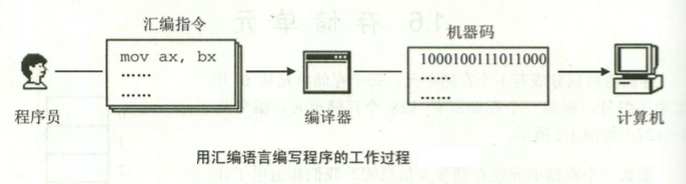
\includegraphics[width=3.5in]{slide01/images/asm_process}
  \end{figure}
\end{frame}
% 
\begin{frame}\ft{存储单元}
  存储器被划分为若干个存储单元,每个存储单元从$0$开始顺序编号。

  \begin{exam}{}
    假设有一个存储器,编号从$0\sim 127$,如下图:
  \begin{figure}
    \centering
    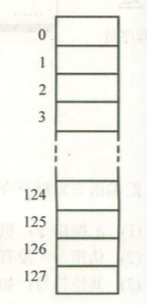
\includegraphics[width=1in]{slide01/images/cunchudanyuan}
  \end{figure}
  \end{exam}
\end{frame}
% 
\begin{frame}\ft{存储单元}

  \begin{defn}[]{}
    \begin{itemize}
    \item 计算机的最小信息单位是Bit,也就是一个二进制位。
    \item 8个Bit组成1个Byte,即一个字节。一个存储单元可存储一个字节。
    \item[] 若一个存储器有128个存储单元,它可以存储128个字节。
    \item 存储器的容量以字节为最小单位来计算。
    \item[] 对于拥有128个存储单元的存储器,其容量为128个字节。 
    \end{itemize}
  \end{defn}


  对于大容量的存储器,还用以下单位来计算容量(以下用B来代表Byte):
  $$
  \begin{array}{ll}
    1KB=2^{10}B=1024B, & 1MB=1025KB, \\
    1GB=1024KB, & 1TB=1025GB, \\
  \end{array}
  $$
\end{frame}
% 
\begin{frame}\ft{CPU对存储器的读写}
  \begin{itemize}
  \item CPU要从内存中读数据,首先要指定单元地址。也就是说要先确定要读哪个单元中的内容。\\[0.1in]
  \item 存储器不止一种。CPU在读写数据时还要指明,对哪一个存储器进行操作,进行哪种操作,是从中读取数据,还是向里面写入数据。

  \end{itemize}
\end{frame}
% 
\begin{frame}\ft{CPU对存储器的读写}
  CPU要想进行数据的读写,必须与外部器件(芯片)进行以下3类信息的交互: 

  \begin{itemize}
  \item 存储单元的地址\red{(地址信息)};\\[0.1in]
  \item 器件的选择,读或写的命令\red{(控制信息)};\\[0.1in]
  \item 读或写的数据\red{(数据信息)}。

  \end{itemize}
\end{frame}
% 
\begin{frame}\ft{CPU对存储器的读写}
  \begin{question}{}
    CPU通过什么将地址、数据和控制信息传给存储器芯片呢?
  \end{question} \pause 
  
  计算机传输的信息都是电信号,电信号当然要用导线传送。

  \begin{defn}[总线]{}
    在计算机中专门有连接CPU和其它芯片的导线,通常称为总线。根据传送信息的不同,从逻辑上分为三类: 

    \begin{itemize}
    \item 地址总线 
    \item 控制总线 
    \item 数据总线
    \end{itemize}
  \end{defn}
\end{frame}
% 
\begin{frame}\ft{CPU从内存中读取数据}
  \begin{exam}[]{}
    \begin{figure}
      \centering
      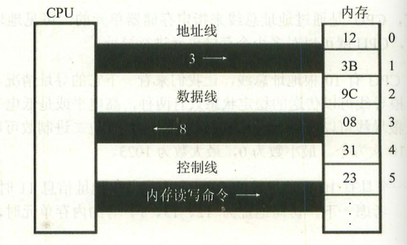
\includegraphics[width=2.5in]{slide01/images/cpu_read}
    \end{figure}
    \begin{enumerate}
    \item CPU通过地址总线将地址信息$3$发出;
    \item CPU通过控制总线发出内存读命令,选中存储器芯片,并通知它,将要从中读取数据;
    \item 存储器将$3$号单元的数据$8$通过数据总线送入CPU。
    \end{enumerate}
  \end{exam}
\end{frame}
% 
\begin{frame}\ft{CPU对存储器的读写}
  写操作与读操作的步骤类似。如向$3$号单元写入数据26。\vspace{0.1in}

  \begin{enumerate}
  \item CPU通过地址总线将地址信息$3$发出;
  \item CPU通过控制总线发出内存写命令,选中存储器芯片,并通知它,将要从中写入数据;
  \item CPU通过数据总线将数据$26$送入内存的$3$号单元中。
  \end{enumerate}
\end{frame}
% 
\begin{frame}\ft{CPU对存储器的读写}
  \begin{question}{}
    我们知道了CPU如何进行数据的读写。那么,我们又如何命令计算机进行数据的读写呢?
  \end{question}\pause \vspace{0.1in}

  要让计算机工作,应向它输入能驱动其进行工作的电平信息,即机器码。\vspace{0.1in}

  \begin{enumerate}
  \item[] 机器指令:1010 0001 0000 0011 0000 0000
  \item[] 汇编指令:mov ax, [3]
  \item[] 含义:传送3号单元的内容入ax。
  \end{enumerate}
\end{frame}

\begin{frame}\ft{地址总线}
  \begin{itemize}
  \item 
    CPU通过地址总线指定存储器单元。由此可见,地址总线能传送多少个不同的信息,CPU就可以对多少个存储单元进行寻址。\pause \\[0.1in]
  \item 
    现假设一个CPU有10根地址总线,可以传送10位二进制数据,共$2^{10}$个不同数据,最小为$0$,最大为$1023$。\pause \\[0.1in]
  \item 
    一个CPU有$N$根地址线,则称CPU的地址总线的宽度为$N$,最多可以寻找$2^N$个内存单元。
  \end{itemize}
\end{frame}
% 
\begin{frame}\ft{地址总线}

  \begin{figure}
    \centering
    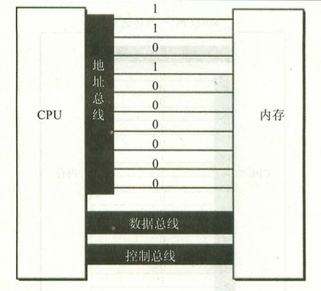
\includegraphics[width=2.5in]{slide01/images/dizhizongxian}
    \caption{地址总线发送的地址信息}
  \end{figure}

\end{frame}
% 
\begin{frame}\ft{数据总线}
  
  CPU与内存和其它器件之间的数据传输通过数据总线来进行。数据总线的宽度决定了CPU与外界的数据传输速度。 
\end{frame}

\begin{frame}\ft{数据总线}

  \begin{figure}
    \centering
    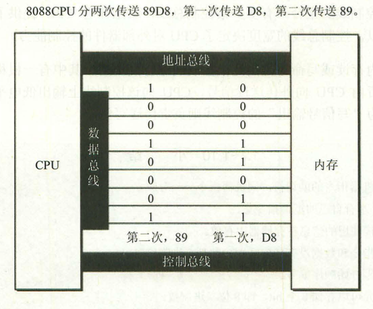
\includegraphics[width=2.5in]{slide01/images/shujuzongxian1}
    \caption{8根数据总线一次可传输一个字节}
  \end{figure}

\end{frame}
% 
\begin{frame}\ft{数据总线}

  \begin{figure}
    \centering
    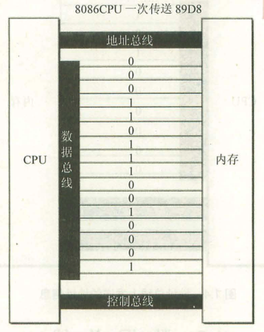
\includegraphics[width=2.in]{slide01/images/shujuzongxian2}
    \caption{16根数据总线一次可传输两个字节}
  \end{figure}

\end{frame}

\begin{frame}\ft{控制总线}
  
  CPU对外部器件的控制通过控制总线来进行。有多少根控制总线,就意味着CPU提供了对外部器件的多少种控制。因此,控制总线的宽度决定了CPU对外部器件的控制能力。 

\end{frame}

\begin{frame}\ft{寄存器}
  一个典型的CPU由运算器、控制器、寄存器等器件构成,这些器件通过内部总线相连。 内部总线实现CPU内部各个器件之间的联系,而外部总线实现CPU与主板上其它器件的联系。 

  在CPU中:
  \begin{itemize}
  \item 运算器进行信息处理;
  \item 寄存器进行信息存储;
  \item 控制器控制各种器件进行工作;
  \item 内部总线连接各种器件,在它们之间进行数据的传送。
  \end{itemize}
\end{frame}
% 
\begin{frame}\ft{寄存器}
  寄存器是CPU中程序员可以用指令读写的部件,程序员通过改变各种寄存器中的内容来实现对CPU的控制。\vspace{0.1in}

  不同的CPU,寄存器的个数、结构不尽相同。8086CPU有14个寄存器,每个寄存器都有一个名称,分别是
  $$
  \mbox{AX、BX、CX、DX、SI、DI、SP、BP、IP、CS、SS、DS、ES、PSW。}
  $$
\end{frame}

\begin{frame}\ft{通用寄存器}
  8086CPU的所有寄存器都是16位的,可以存放两个字节。\vspace{0.1in}

  AX、BX、CX、DX这四个寄存器通常用来存放一般性的数据,被称为通用寄存器。

  \begin{figure}
    \centering
    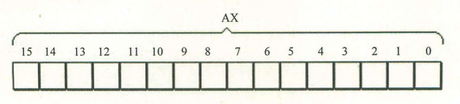
\includegraphics[width=3.5in]{slide01/images/tongyongjicunqi1}
    \caption{16位寄存器的逻辑结构}
  \end{figure}


\end{frame}

\begin{frame}\ft{通用寄存器}
  \begin{figure}
    \centering
    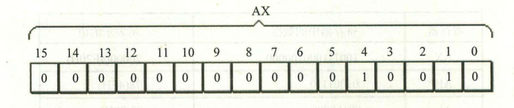
\includegraphics[width=3.5in]{slide01/images/tongyongjicunqi2}
    \caption{$(10010)_2$在寄存器AX中的存储}
  \end{figure}
  
  \begin{figure}
    \centering
    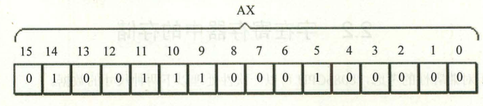
\includegraphics[width=3.5in]{slide01/images/tongyongjicunqi3}
    \caption{$(100111000100000)_2$在寄存器AX中的存储}
  \end{figure}
\end{frame}
% 
% 
% 
\begin{frame}\ft{通用寄存器}
  \begin{figure}
    \centering
    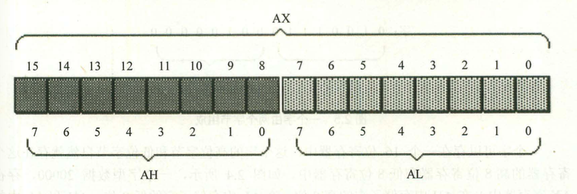
\includegraphics[width=3.5in]{slide01/images/tongyongjicunqi4}
    \caption{16位寄存器可分为两个8位寄存器}
  \end{figure}
\end{frame}

\begin{frame}\ft{几条汇编指令}
  \begin{figure}
    \centering
    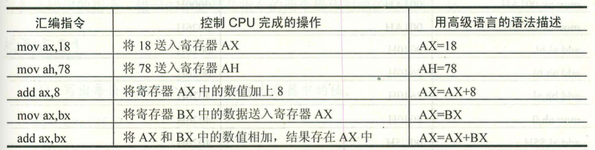
\includegraphics[width=4.5in]{slide01/images/huibianzhiling1}
    \caption{汇编指令举例}
  \end{figure}
\end{frame}

% \begin{frame}\ft{物理地址}
%   CPU访问内存单元时,要给出内存单元的地址。所有的内存单元构成的存储空间是一个一维的线性空间,每一个内存单元在这个空间中都有唯一的地址,称为物理地址。\vspace{0.1in}

%   CPU通过地址总线送入存储器的,必须是一个内存单元的物理地址。在CPU向地址总线上发出物理地址之前,必须要在内部先形成这个物理地址。不同的CPU可以有不同的形成物理地址的方式。
% \end{frame}

% \begin{frame}\ft{16位结构的CPU}
%   16位结构描述了一个CPU具有以下几个方面的结构特性。\vspace{0.1in}
%   
%   \begin{itemize}
%   \item 运算器一次最多可以处理16位的数据;\\[0.1in]
%   \item 寄存器的最大宽度为16位;\\[0.1in]
%   \item 寄存器与运算器之间的通路是16位。
%   \end{itemize}
% \end{frame}
% 
% \begin{frame}\ft{8086CPU给出物理地址的方法}
%   8086CPU有20位地址总线,可以传送20位地址,达到1MB寻址能力。\vspace{0.1in}
%   
%   同时8086CPU是16位结构,在内部一次处理、传输、暂存的地址是16位。
%   \vspace{0.1in}
%   
%   从8086CPU的内部结构来看,若将地址从内部简单出发,只能送出16位的地址,表现出的寻址能力只有64KB。\pause 
%   \vspace{0.1in}
%   
%   \red{8086CPU采用一种在内部用两个16位地址合成的方法来形成一个20位的物理地址。}
% \end{frame}
% 
% \begin{frame}\ft{8086CPU给出物理地址的方法}
%   \begin{figure}
%     \centering
%     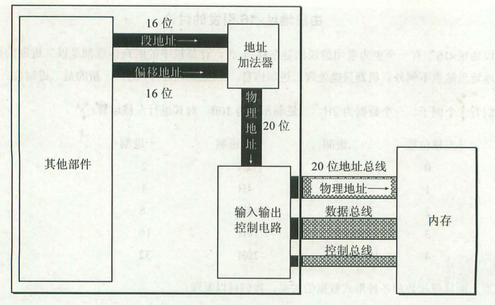
\includegraphics[width=4in]{slide01/images/xunzhi}
%     \caption{8086CPU相关部件的逻辑结构}
%   \end{figure}
% \end{frame}
% 
% \begin{frame}\ft{8086CPU给出物理地址的方法}
%   \begin{figure}
%     \centering
%     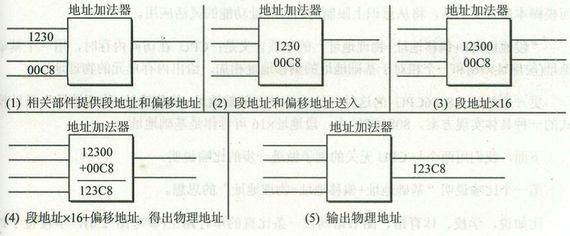
\includegraphics[width=4in]{slide01/images/xunzhi1}
%     \caption{地址加法器的工作过程(物理地址=段地址$\times$16+偏移地址)}
%   \end{figure}
%   
% \end{frame}
%% 
% \begin{frame}\ft{段的概念}
%   \begin{figure}
%     \centering
%     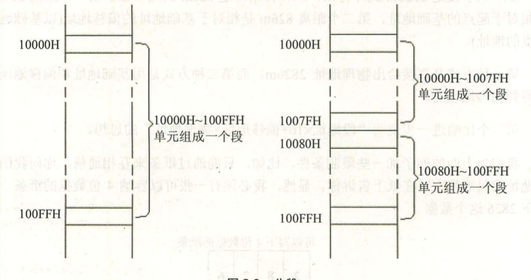
\includegraphics[width=4in]{slide01/images/duan}
%     \caption{内存并没有分段,段的划分来自于CPU,由于8086CPU用“基础地址(段地址$\times$16)+偏移地址”的方式给出内存单元的物理地址,使得我们可以用分段的方式来管理内存。}
%   \end{figure}
% \end{frame}
% 
% \begin{frame}\ft{段寄存器}
%   8086CPU在访问内存时由相关部件提供内存单元的段地址和偏移地址,送入地址加法器合成物理地址。\vspace{0.1in}
%   
%   段地址在8086CPU的段寄存器中存放。8086CPU有4个段寄存器:CS、DS、SS、ES。\vspace{0.1in}
%   
%   8086CPU访问内存时由这四个段寄存器提供内存单元的段地址。
% \end{frame}
% 
% \begin{frame}\ft{CS和IP}
%   CS和IP是8086CPU中两个最关键的寄存器,指示CPU当前要读取指令的地址。
%   \vspace{0.1in}
%   
%   CS为代码段寄存器,IP为指令指针寄存器。
%   \vspace{0.1in}
%   
%   设CS的内容为$M$,IP的内容为$N$,则8086CPU将从内存$M\times16+N$单元开始,读取一条指令并执行。\pause \vspace{0.2in}
%   
%   \red{以下展示8086CPU读取、执行命令的工作原理:}
% \end{frame}
% 
% \begin{frame}\ft{CS和IP}
%   
%   \begin{figure}
%     \centering
%     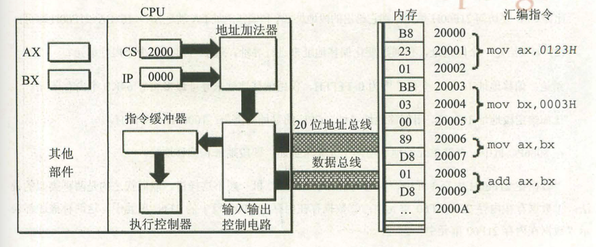
\includegraphics[width=4.5in]{Tikz/csip1}
%     \caption{初始状态:CPU将从内存2000:0000处读取指令}
%   \end{figure}
%   
% \end{frame}
% 
% \begin{frame}\ft{CS和IP}
%   \begin{figure}
%     \centering
%     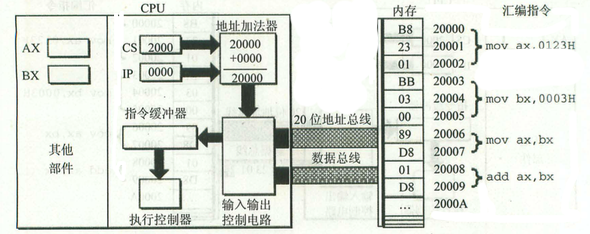
\includegraphics[width=4.5in]{Tikz/csip2}
%     \caption{CS、IP中的内容送入地址加法器,形成物理地址}
%   \end{figure}
%   
% \end{frame}
% 
% 
% \begin{frame}\ft{CS和IP}
%   \begin{figure}
%     \centering
%     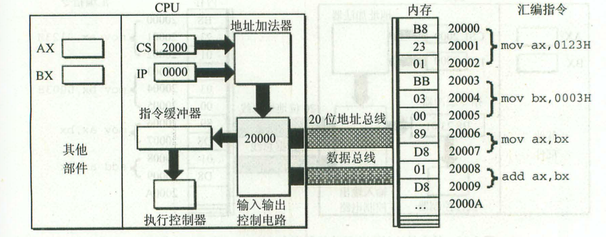
\includegraphics[width=4.5in]{Tikz/csip3}
%     \caption{地址加法器将物理地址送至输入输出控制电路}
%   \end{figure}
%   
% \end{frame}
% 
% \begin{frame}\ft{CS和IP}
%   \begin{figure}
%     \centering
%     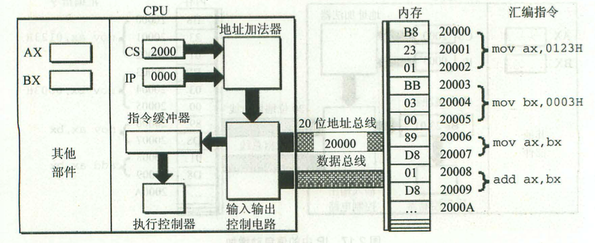
\includegraphics[width=4.5in]{Tikz/csip4}
%     \caption{输入输出控制电路将物理地址送上地址总线}
%   \end{figure}
%   
% \end{frame}
% 
% \begin{frame}\ft{CS和IP}
%   \begin{figure}
%     \centering
%     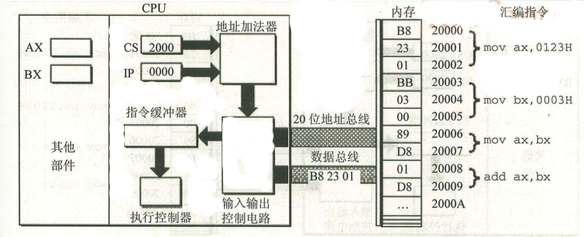
\includegraphics[width=4.5in]{Tikz/csip5}
%     \caption{将内存20000H单元开始存放的机器指令B8~23~01通过数据总线送入CPU}
%   \end{figure}
%   
% \end{frame}
% 
% 
% \begin{frame}\ft{CS和IP}
%   \begin{figure}
%     \centering
%     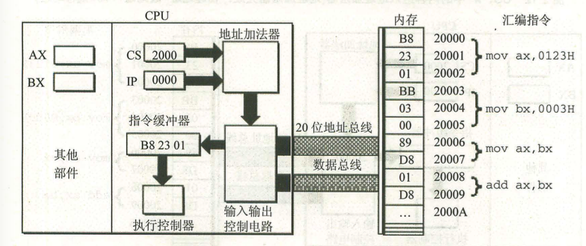
\includegraphics[width=4.5in]{Tikz/csip6}
%     \caption{输入输出控制电路将机器指令B8~23~01送入指令缓冲器}
%   \end{figure}
%   
% \end{frame}
% 
% \begin{frame}\ft{CS和IP}
%   \begin{figure}
%     \centering
%     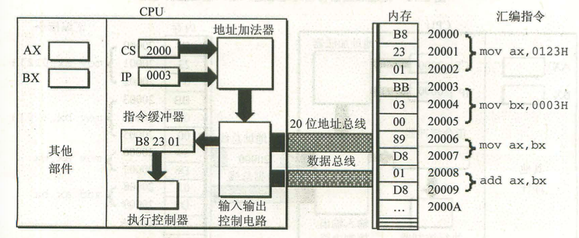
\includegraphics[width=4.5in]{Tikz/csip7}
%     \caption{IP中的值自动增加:读取一条指令后,IP中的值自动增加,以使CPU可以读取下一条指令。因当前读入的指令B8~23~01为3个字节,故IP中的值加3。}
%   \end{figure}
%   
% \end{frame}
% 
% 
% \begin{frame}\ft{CS和IP}
%   \begin{figure}
%     \centering
%     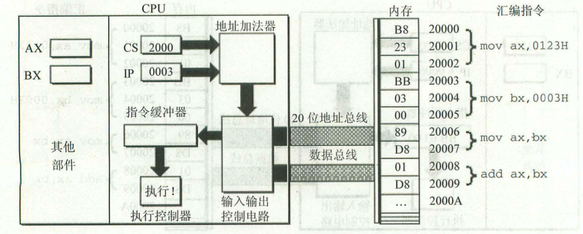
\includegraphics[width=4.5in]{Tikz/csip8}
%     \caption{执行控制器执行指令B8~23~01,即mov ax, 0123H}
%   \end{figure}
%   
% \end{frame}
% 
% \begin{frame}\ft{CS和IP}
%   \begin{figure}
%     \centering
%     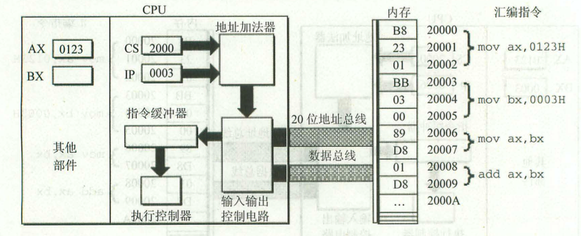
\includegraphics[width=4.5in]{Tikz/csip9}
%     \caption{指令B8~23~01被执行后AX中的内容为0123H,此时CPU将从内存单元2000:0003处读取指令。}
%   \end{figure}
%   
% \end{frame}
% 
% \begin{frame}\ft{CS和IP}
%   \begin{figure}
%     \centering
%     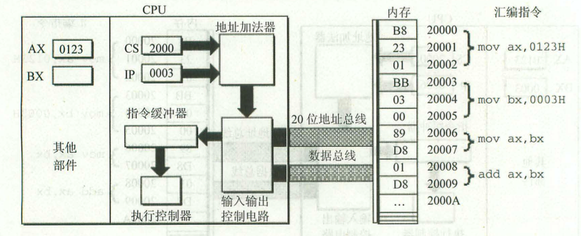
\includegraphics[width=4.5in]{Tikz/csip9}
%     \caption{CS:2000H,IP:0003H,CPU将读取指令BB~03~00}
%   \end{figure}
%   
% \end{frame}
% 
% \begin{frame}\ft{CS和IP}
%   \begin{figure}
%     \centering
%     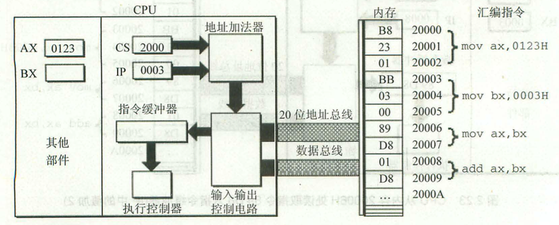
\includegraphics[width=4.5in]{Tikz/csip10}
%     \caption{CPU读取指令BB~03~00入指令缓冲器,IP中的值加3。}
%   \end{figure}
%   
% \end{frame}
% 
% 
% 
% 
% \begin{frame}\ft{CS和IP}
%   \begin{figure}
%     \centering
%     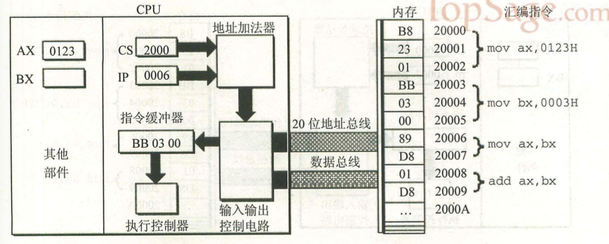
\includegraphics[width=4.5in]{Tikz/csip11}
%     \caption{执行指令BB~03~00,即mov bx, 0003H}
%   \end{figure}
%   
% \end{frame}
% 
% 
% \begin{frame}\ft{CS和IP}
%   \begin{figure}
%     \centering
%     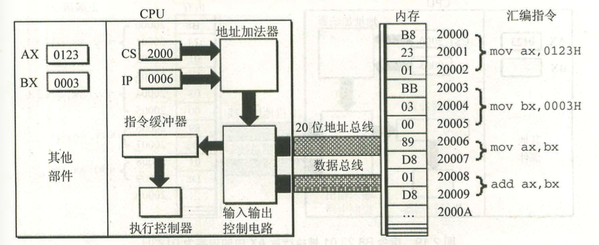
\includegraphics[width=4.5in]{Tikz/csip12}
%     \caption{CPU从内存20006H处读取指令89~D8如指令缓冲器,IP中的值加2。}
%   \end{figure}
%   
% \end{frame}
% 
% \begin{frame}\ft{CS和IP}
%   \begin{figure}
%     \centering
%     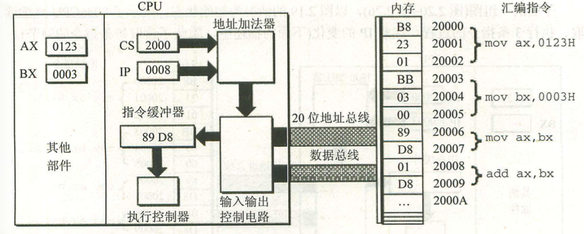
\includegraphics[width=4.5in]{Tikz/csip13}
%     \caption{执行指令89~D8,即mov ax, bx后,AX中的内容为0003H}
%   \end{figure}
%   
% \end{frame}
% 
% \begin{frame}\ft{CS和IP}
%   \begin{figure}
%     \centering
%     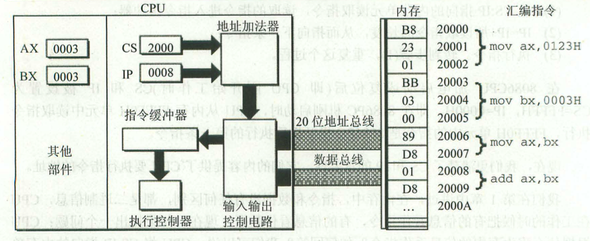
\includegraphics[width=4.5in]{Tikz/csip14}
%     \caption{CPU从内存20008H处读取指令01~D8如指令缓冲器,IP中的值加2。}
%   \end{figure}
%   
% \end{frame}
% 
% \begin{frame}\ft{CS和IP}
%   \begin{figure}
%     \centering
%     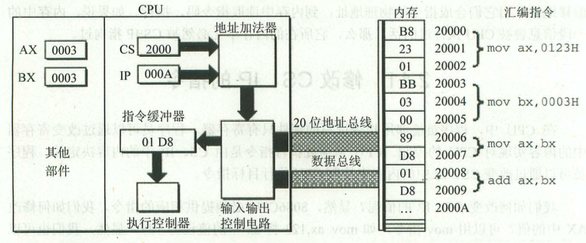
\includegraphics[width=4.5in]{Tikz/csip15}
%     \caption{执行指令01~D8,即add ax, bx后,AX中的内容为0006H}
%   \end{figure}
% \end{frame}
% 
% \begin{frame}\ft{CS和IP}
%   8086CPU的工作过程:\vspace{0.1in}
%   
%   \begin{itemize}
%   \item[(1)] 从CS:IP指向的内存单元读取指令,读取的指令进入指令缓冲器;\\[0.1in]
%   \item[(2)] IP=IP+所读取指令的长度,从而指向下一条指令;\\[0.1in]
%   \item[(3)] 执行指令。转至步骤(1),重复整个过程。
%   \end{itemize}
% \end{frame}
% 
% \begin{frame}\ft{CS和IP}
%   CPU刚开始工作时,CS和IP被设置为CS=FFFFH,IP=0000H,即开机时,CPU从内存FFFF0H单元中读取指令执行,FFFF0H单元中的指令是开机后执行的第一条指令。
% \end{frame}
% 
% 
% 
